\documentclass[10pt,aspectratio=169]{beamer}
\usepackage{../../common/foundationsmacro-beamer}
\usepackage{pgfplots}
\pgfplotsset{compat=1.18}
\usepackage{tikz}
\usetikzlibrary{calc,arrows.meta,decorations.pathreplacing,patterns,shapes,positioning,intersections,math,backgrounds,plotmarks,matrix}
\usepackage{booktabs}
\usepackage{bm}

% Preserve the original diagram color name using the shared course palette.
\colorlet{TitleBlue}{MacroBlue}

\title[Economic Growth]{Chapter III: Economic Growth}

\author[Bueren]{Jes\'{u}s Bueren}
\institute{}
\date{}

\begin{document}
\begin{frame}[plain]
    \titlepage
\end{frame}

\section{Facts on Growth}
\begin{frame}{Why Study Economic Growth?}

\begin{itemize}
  \item As we saw in chapter I, GDP shapes to a large extent living standards.
  \itemvso Even \textbf{small differences} in gdp growth rates create \textbf{huge income gaps} over time.
  \itemvso Rule of thumb: if gdp grows at $g\%$ per year,
  $$\text{Doubling time} \approx \frac{70}{g} \text{ years.}$$
\item Examples:
    \begin{itemize}
        \itemvso \textbf{South Korea vs.\ Afghanistan}: similar income per capita in the 1960s, but sustained faster growth made Korea one of the richest countries in Asia while Afghanistan became x10 poorer.
        \itemvso \textbf{Poland vs.\ Portugal}: Portugal was nearly x3 richer in GDP per capita in the early 1990s, yet Poland’s consistently higher growth has allowed it to surpass Portugal.
    \end{itemize}
    \itemvso Understanding what drives growth helps us understand why some countries prosper while others fall behind.
\end{itemize}
\end{frame}


\begin{frame}{GDP per Capita Since 1865}
\centering
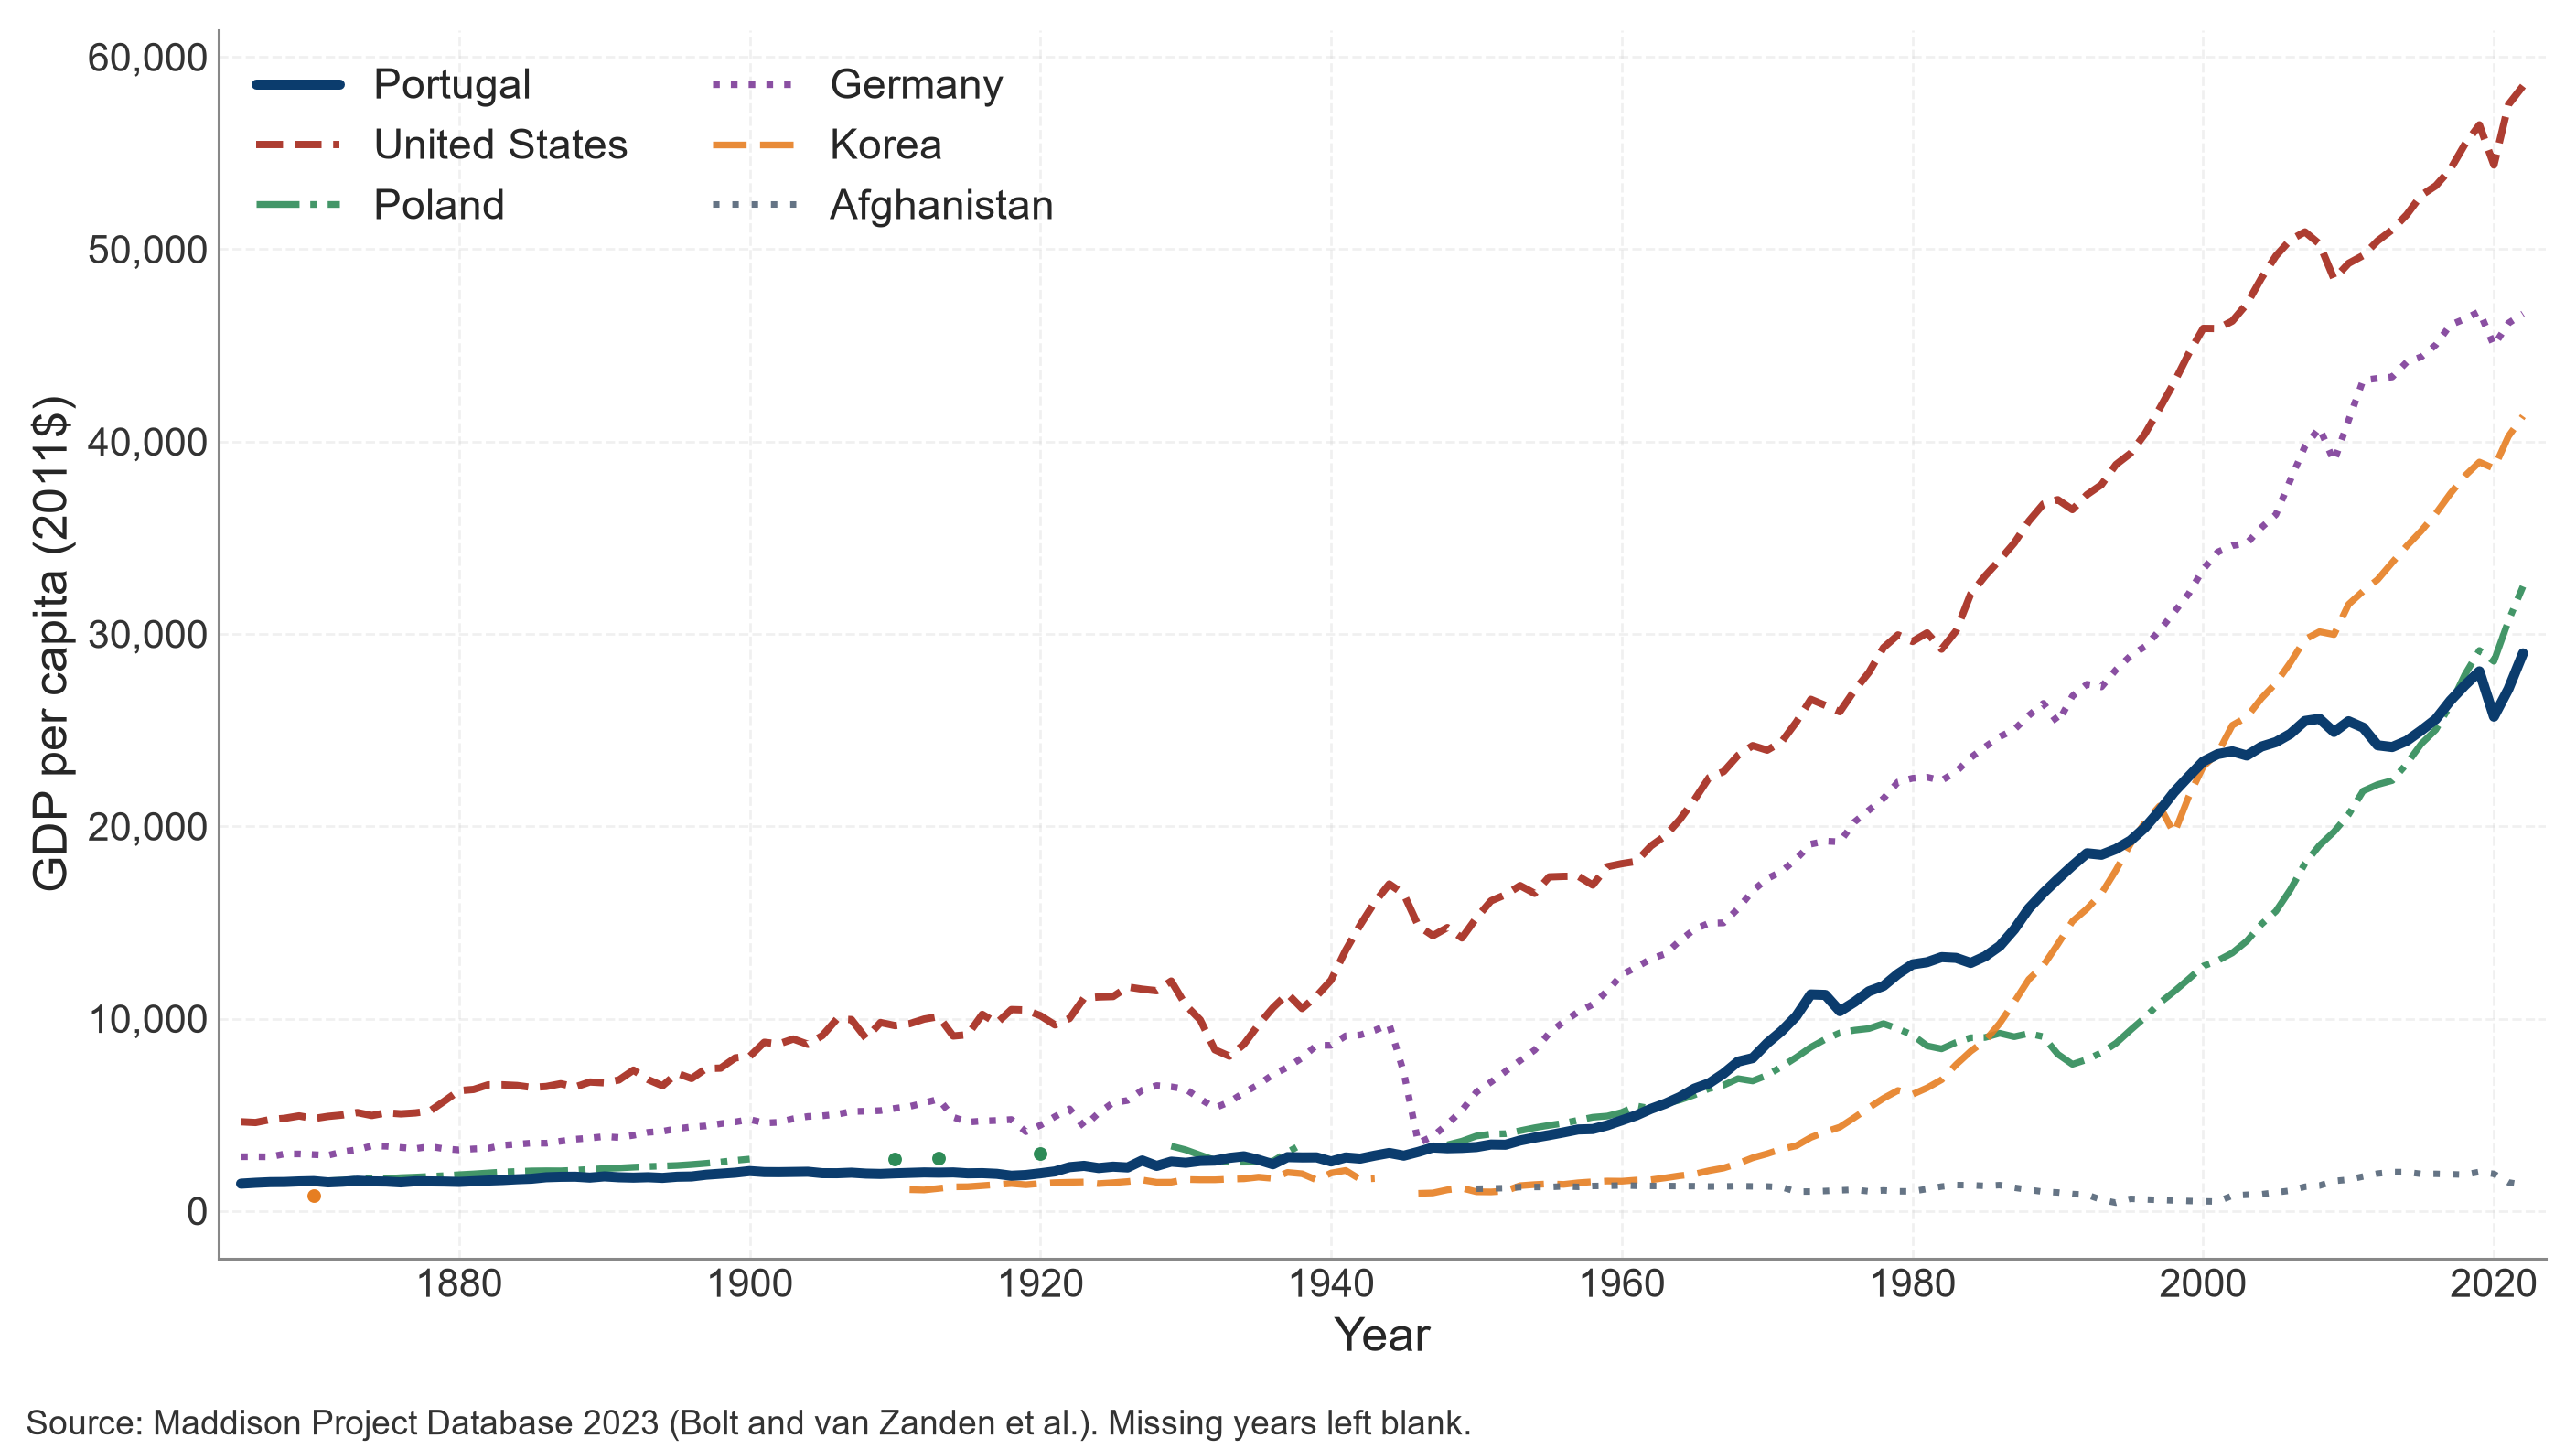
\includegraphics[width=0.98\textwidth,height=0.9\textheight,keepaspectratio]{figures/portugal_gdppc_1865.png}
\end{frame}


\section{The Solow Growth Model}
\begin{frame}{The Solow--Swan Model}

\begin{itemize}
    \item The Solow--Swan (1956) model is a simple model to study long-run economic growth.
    \itemvso It provides a  description of how capital accumulation and technology shape GDP per capita.
    \itemvso In contrast to the model that we saw in chapter 2, the capital stock is going to be determined within the model.
    \itemvso Let's see the main ingredients.
\end{itemize}

\end{frame}


\subsection{Production}
% Slide 1: Production Function
%-------------------- SLIDE 1 --------------------
\begin{frame}{Production Function}

\begin{itemize}
    \item A production function tells us how inputs become output:
    \[
        Y = F(K,L)
    \]
    \vspace{-.3cm}
    \itemvso Inputs:
        \begin{itemize}
            \itemvso $K$: capital (machines, buildings, equipment)
            \itemvso $L$: labor (hours of work)
        \end{itemize}

\end{itemize}

\end{frame}


\subsection{Consumption and Investment}
\begin{frame}{Consumption and Investment}
\begin{itemize}
\item The economy is closed and there is no government and population is constant: $\bar{L}$

    \itemvso The national income identity simplifies to:
    \[
        Y = C + I
    \]
    \vspace{-.3cm}
    \item All output is either consumed or invested.
\end{itemize}

\end{frame}

\begin{frame}{Savings and Investment}
\begin{itemize}
\item The savings rate is exogenous and constant:
\[
    \frac{S}{Y} = s.
\]

    \itemvso Income is equal to output: \(Y\) is both.
    \itemvso Savings: \(S = Y - C\).
    \itemvso Savings rate: \(\frac{Y-C}{Y} = s\).
    \itemvso In a closed economy, savings equal investment: \(S = I\).
\end{itemize}
\end{frame}

\subsection{Capital Accumulation}
\begin{frame}{Depreciation and Capital Accumulation}

\begin{itemize}
\item In contrast to the previous chapter, this model is going to be dynamic.
\itemvso The capital stock depreciates at a constant rate \(\delta\).
    \itemvso Capital wears out: machines break, buildings deteriorate, technology becomes obsolete.
    \itemvso Each period, a fraction \(\delta\) of the capital stock loses its productive value.

\[
    K_{t+1} = (1 - \delta)K_t + I_t
\]

    \itemvso \((1 - \delta)K_t\): capital that survives depreciation.
    \itemvso \(I_t\): new capital created through investment.
\end{itemize}

\end{frame}
\begin{frame}{Capital Accumulation: A Numerical Example}

\begin{itemize}
    \item Consider an economy with initial capital $K_0 = 1,000$ units, constant investment $I_t = 200$ units, and depreciation rate $\delta = 0.10$.
    \itemvso How does the capital stock evolve?
\end{itemize}

\vspace{0.3cm}

\begin{center}
\begin{tabular}{ccccc}
\toprule
\textbf{Time } $\mathbf{t}$ & \textbf{Capital } $\mathbf{K_t}$ & \textbf{Investment } $\mathbf{I_t}$ & \textbf{Depreciation } $\boldsymbol{\delta K_t}$ & \textbf{Change } $\boldsymbol{\Delta K_{t+1}}$ \\
\midrule
0 & 1,000 & 200 & 100 & 100 \\
1 & 1,100 & 200 & 110 & 90 \\
2 & 1,190 & 200 & 119 & 81 \\
3 & 1,271 & 200 & 127 & 73 \\
4 & 1,344 & 200 & 134 & 66 \\
5 & 1,410 & 200 & 141 & 59 \\
\bottomrule
\end{tabular}
\end{center}

\vspace{0.3cm}

\begin{itemize}
    \itemvso Each period: $\Delta K_{t+1} = I_t - \delta K_t$.
    \itemvso Net investment decreases over time as depreciation rises with the capital stock.
\end{itemize}

\end{frame}
\section{Solving the Model}

\begin{frame}{Per Capita Production Function}

We rewrite the production function in per-capita terms. Define:
\[
y \equiv \frac{Y}{\bar{L}}, \qquad 
k \equiv \frac{K}{\bar{L}}
\]
where \(y\) is GDP per capita and \(k\) is capital per worker.

\bigskip

Starting from the aggregate production function:
\[
y = \frac{F(K,\bar{L})}{\bar{L}} = F\!\left(\frac{K}{\bar{L}},\,1\right) \equiv f(k)
\]

\begin{itemize}
    \item The first step substitutes \(Y = F(K,\bar{L})\) from the aggregate production function.
    \itemvso Because of constant returns to scale, scaling both inputs by \(1/\bar{L}\) leaves output per worker well-defined.
    \itemvso We define the per-capita production function \(f(k)\) as the output produced by one worker with \(k\) units of capital.
\end{itemize}

\end{frame}

\begin{frame}{Dynamics of Capital per Worker}

We want to understand how capital per worker evolves over time:
\[
k_{t+1} \equiv \frac{K_{t+1}}{\bar{L}}
\]

Start from the capital accumulation equation:
\[
K_{t+1} = (1-\delta)K_t + I_t
\]

Use:
\[
I_t = sY_t
\]

Combining these:
\[
k_{t+1}
= (1-\delta)k_t + s y_t
\]

\[
\Rightarrow 
\Delta k_{t+1} 
=(1-\delta)k_t + s y_t-k_t= s f(k_t) - \delta k_t
\]

\end{frame}

\begin{frame}{Interpretation of the Dynamics}

The evolution of capital per worker depends on two opposing forces:

\bigskip

\begin{itemize}
    \item \textbf{Investment per worker:} 
    \[
    \underbrace{s f(k)}_{\text{adds to }k}
    \]
    
    \item \textbf{Depreciation:}
    \[
    \underbrace{\delta k}_{\text{subtracts from }k}
    \]
    Depreciation consumes part of the capital stock.
\end{itemize}

\bigskip

Thus:
\[
\Delta k > 0 \iff s f(k) > \delta  k
\]
\[
\Delta k < 0 \iff s f(k) < \delta  k
\]

\end{frame}

\begin{frame}{Solving the model}

\begin{center}
\begin{tikzpicture}[scale=0.9, samples=200]
    % --- PARAMETERS ---
    \def\kmax{7.5}
    \def\ymax{5.5}
    \def\A{2.5}
    \def\alpha{0.35}
    \def\s{0.4}
    \def\kss{5}
    \def\slope{\s*\A*\kss^(\alpha-1)} 

    % --- SHADED REGIONS ---
    % Green Region (Investment > Depreciation)
    \fill[green!20, domain=0:\kss] 
        plot (\x, {\s * \A * \x^\alpha}) -- plot[domain=\kss:0] (\x, {\slope * \x}) -- cycle;
    
% Red Region (Depreciation > Investment) - Now extends to \kmax
    \fill[red!20, domain=\kss:\kmax] 
        plot (\x, {\s * \A * \x^\alpha}) -- plot[domain=\kmax:\kss] (\x, {\slope * \x}) -- cycle;
    % --- AXES ---
    \draw[->, thick] (0,0) -- (\kmax,0) node[right] {Capital ($k$)};
    \draw[->, thick] (0,0) -- (0,\ymax) node[above] {Output, Investment, Depreciation};

    % --- PLOTS ---
    \draw[thick, blue, domain=0:\kmax] plot (\x, {\A * \x^\alpha}) node[right] {$y = f(k)$};
    \draw[thick, teal, domain=0:\kmax] plot (\x, {\s * \A * \x^\alpha}) node[right] {$s y$};
    \draw[thick, red, domain=0:\kmax] plot (\x, {\slope * \x}) node[right] {$\delta k$};

    % --- STEADY STATE MARKERS ---
    \pgfmathsetmacro{\yss}{\A * \kss^\alpha}
    \pgfmathsetmacro{\iss}{\s * \yss}

    \draw[dashed] (\kss, \yss) -- (\kss, 0) node[below=5pt] {$k_{ss}$};
    \draw[dashed] (\kss, \yss) -- (0, \yss) node[left] {$y_{ss}$};
    \draw[dashed] (\kss, \iss) -- (0, \iss) node[left] {$i_{ss}$};

    \fill[black] (\kss, \iss) circle (2pt);
    \fill[black] (\kss, \yss) circle (2pt);

    % --- DYNAMIC ARROWS ON X-AXIS ---
    % Arrow pointing right (towards kss)
    \draw[->, ultra thick, green!60!black] (1, -0.5) -- (2.5, -0.5) node[midway, below] {$\Delta k > 0$};
    % Arrow pointing left (towards kss)
    \draw[->, ultra thick, red!60!black] (7, -0.5) -- (5.5, -0.5) node[midway, below] {$\Delta k < 0$};

\end{tikzpicture}
\end{center}

\end{frame}

\begin{frame}{The Steady State}

The steady state is where capital per worker does not change:
\[
k_{t+1} = k_t = k_{ss}
\]

Condition:
\[
s f(k_{ss}) = \delta k_{ss}
\]

\bigskip

\begin{itemize}
    \item If $k < k_{ss}$: investment exceeds depreciation+dilution $\Rightarrow k$ rises.
    \itemvso If $k > k_{ss}$: investment is too small to sustain the level of capital $\Rightarrow k$ falls.
    \itemvso The economy converges to $k_{ss}$ over time.
\end{itemize}

\end{frame}


\begin{frame}{Closed-Form Steady State: Cobb--Douglas}

If:
\[
y = A k^\alpha
\]

where $A$ denotes a productivity parameter driving higher or lower output given a quantity of capital.\\
\vspace{0.3cm}
Then, steady state satisfies:
\[
s A k_{ss}^\alpha = \delta k_{ss}
\]

Solving:
\[
k_{ss} = 
\left(
\frac{s A}{\delta}
\right)^{\frac{1}{1-\alpha}}
\]

\[
y_{ss} = A
\left(
\frac{s A}{\delta}
\right)^{\frac{\alpha}{1-\alpha}}
\]

\end{frame}

\section{Rich and Poor Countries}
\begin{frame}{Why are poor countries poor?}
\begin{itemize}
\item Now let's use our model to try to rationalize differences in GDP per capita across countries and what could be its main drivers.
\itemvso Let's imagine that we have two economies:
\begin{itemize}
\item Poor economy:  $s_{\text{poor}}, A_{\text{poor}}$
\item Rich economy:  $s_{\text{rich}}, A_{\text{rich}}$
\end{itemize}
\itemvso Assume that the depreciation rate is equal across these two countries.
\itemvso The ratio of GDP per capita across these two economies is given by:
\begin{align*}
\dfrac{y_{\text{rich}}}{y_{\text{poor}}}&=\Bigg(\dfrac{A_{\text{rich}}}{A_{\text{poor}}}\Bigg)^{\dfrac{1}{1-\alpha}} \Bigg(\dfrac{s_{\text{rich}}}{s_{\text{poor}}}\Bigg)^{\dfrac{\alpha}{1-\alpha}}
\end{align*}
\end{itemize}
\end{frame}


\begin{frame}{Why are poor countries poor?}{The Role of Investment vs Productivity differences}
\begin{itemize}
\item With $\alpha=1/3$, we get:
\begin{align*}
\dfrac{y_{\text{rich}}}{y_{\text{poor}}}&=\Bigg(\dfrac{A_{\text{rich}}}{A_{\text{poor}}}\Bigg)^{3/2} \Bigg(\dfrac{s_{\text{rich}}}{s_{\text{poor}}}\Bigg)^{1/2}
\end{align*}
\item The richest countries in the world have a GDP per capita around 70 times larger than poor countries
\itemvso Investment rates are around  28\% in rich countries and 7\% in poor countries 
\itemvso These means that according to the Solow model, differences in savings rate would make rich countries around $\Big( 28/7 \Big)^{1/2}=2$ times richer
\itemvso If poor countries had the productivity of rich countries, they would be 35 times richer! (in contrast to 14 in the previous chapter, why?)
\end{itemize}
\end{frame}

\section{Growth in Solow}
\begin{frame}{Economic Growth in the Solow Model}{Steady State}
\begin{itemize}
\item The Solow model implies convergence to a \textbf{steady state}.
\itemvso In the long run:
\begin{itemize}
    \item Capital and output are constant: $K^*,\, Y^*$.
    \item Output per person is constant:
    \[
    y^* \equiv \frac{Y^*}{\bar{L}}
    \]
    \item Consumption per person is constant:
    \[
    c^* = (1 - s)y^*
    \]
\end{itemize}
\item Long-run growth in $y$ is zero.
\end{itemize}
\end{frame}

\begin{frame}{Economic Growth in the Solow Model}{Transition vs. Data}
\begin{itemize}
\item The model allows for growth only \textbf{during transition}.
\itemvso If $K_0 < K^*$:
\begin{itemize}
    \itemvso Capital accumulates.
    \itemvso Output per person grows temporarily.
\end{itemize}
\itemvso Once $K = K^*$, growth stops.
\itemvso But in the data:
\begin{itemize}
    \itemvso GDP per capita grows persistently over time.
    \itemvso U.S. GDP per capita: $\approx 2\%$ per year for over a century.
\end{itemize}
\end{itemize}
\end{frame}

\begin{frame}{Economic Growth in the Solow Model}{Key Lesson}
\begin{itemize}
\item Capital accumulation cannot explain \textbf{long-run} growth.
\itemvso Diminishing returns to capital imply:
\begin{itemize}
    \item Falling marginal product of capital.
    \item Investment eventually only offsets depreciation.
\end{itemize}
\itemvso Physical capital drives \textbf{medium-run} growth, not long-run growth.
\itemvso Something else must sustain growth.
\end{itemize}
\end{frame}

\section{Economic Experiments}


\begin{frame}{Increase in the Savings Rate}
Suppose an economy in steady state $k^*$ experiences a permanent increase in the savings rate from $s$ to $s'$.

\begin{itemize}
    \itemvso  The investment curve $sf(k)$ rotates upward to $s'f(k)$. For any given level of capital, the economy now saves and invests more.

        \itemvso At the old steady state $k^*$, investment now exceeds depreciation: $s'f(k^*) > \delta k^*$.
        \itemvso This surplus causes the capital stock to grow ($\Delta k > 0$).
        \itemvso As $k$ rises, output $y$ also rises along the production function.

    \itemvso  Growth continues but slows down as the economy approaches $k^{**}$, where $s'f(k^{**}) = \delta k^{**}$.
    \itemvso The levels of capital per worker and output per worker are permanently higher, but the long-run \textit{growth rate} eventually returns to zero.
\end{itemize}
 \end{frame}

\begin{frame}{Increase in Savings Rate}
\begin{center}
\begin{tikzpicture}[scale=0.75, samples=200]
    % --- PARAMETERS ---
    \def\kmax{12.5}
    \def\ymax{7.5}
    \def\A{2.8}
    \def\alpha{0.35}
    \def\sLow{0.35}    
    \def\sHigh{0.55}   
    
    % MANUALLY DEFINE SS FOR PERFECT ALIGNMENT
    \def\kssLow{4.0}   % Original Steady State
    \def\kssHigh{8.0}  % New Steady State (visibly further right)

    % CALCULATE THE SLOPE based on sLow and kssLow 
    % (delta + n) = sLow * A * kssLow^(alpha - 1)
    \pgfmathsetmacro{\slope}{\sLow * \A * (\kssLow^(\alpha-1))}
    
    % CALCULATE THE NEW sHigh required to make kssHigh the exact intersection
    % sHigh = (slope * kssHigh) / (A * kssHigh^alpha)
    \pgfmathsetmacro{\sHighAdj}{(\slope * \kssHigh) / (\A * \kssHigh^\alpha)}

    % --- SHADED REGIONS ---
    % Green Region: From 0 to new SS
    \fill[green!15, domain=0.01:\kssHigh] 
        plot (\x, {\sHighAdj * \A * \x^\alpha}) -- plot[domain=\kssHigh:0.01] (\x, {\slope * \x}) -- cycle;

    % --- AXES ---
    \draw[->, thick] (0,0) -- (\kmax,0) node[right] {$k$};
    \draw[->, thick] (0,0) -- (0,\ymax) node[above] {$y, i$};

    % --- PLOTS ---
    % Production Function
    \draw[thick, blue, domain=0:\kmax] plot (\x, {\A * \x^\alpha}) node[right] {$f(k)$};
    
    % Old Investment Curve
    \draw[thick, teal, domain=0:\kmax, dashed, opacity=0.6] plot (\x, {\sLow * \A * \x^\alpha}) node[right] {$s f(k)$};
    
    % New Investment Curve (using adjusted s to force intersection at kssHigh)
    \draw[ultra thick, teal, domain=0:\kmax] plot (\x, {\sHighAdj * \A * \x^\alpha}) node[right] {$s' f(k)$};
    
    % Depreciation Line
    \draw[thick, red, domain=0:\kmax] plot (\x, {\slope * \x}) node[right] {$\delta k$};

    % --- STEADY STATE MARKERS ---
    % Old SS
    \pgfmathsetmacro{\yssLow}{\A * \kssLow^\alpha}
    \pgfmathsetmacro{\issLow}{\sLow * \yssLow}
    \draw[dashed, gray] (\kssLow, \yssLow) -- (\kssLow, 0) node[below, black] {$k^*$};
    \fill[black] (\kssLow, \issLow) circle (2pt);

    % New SS
    \pgfmathsetmacro{\yssHigh}{\A * \kssHigh^\alpha}
    \pgfmathsetmacro{\issHigh}{\sHighAdj * \yssHigh}
    \draw[dashed] (\kssHigh, \yssHigh) -- (\kssHigh, 0) node[below] {$k^{**}$};
    \fill[black] (\kssHigh, \issHigh) circle (2pt);
    \fill[black] (\kssHigh, \yssHigh) circle (2pt);

    % --- ROTATION & TRANSITION ---
    \draw[->, bend left, thick, orange] (2, 1.2) to node[left, black, scale=0.8] {$s \uparrow$} (2, 1.8);
    \draw[->, ultra thick, orange] (\kssLow + 0.2, -0.6) -- (\kssHigh - 0.2, -0.6) node[midway, below] {Transition};

\end{tikzpicture}
\end{center}
\end{frame}



\begin{frame}{Increase in the Depreciation Rate}
Suppose an economy in steady state $k^*$ faces a permanent increase in the depreciation rate from $\delta$ to $\delta'$.

\begin{itemize}
    \item The investment line $\delta k$ rotates upward (becomes steeper). For every unit of capital, more investment is now required just to maintain the current level.


        \itemvso At the original steady state $k^*$, depreciation now exceeds investment: $\delta' k^* > sf(k^*)$.
        \itemvso The net change in capital becomes negative ($\Delta k < 0$).
        \itemvso The capital stock begins to decline, which in turn reduces output per worker $y$ along the production function.

    \itemvso  The capital stock continues to contract until it reaches $k^{**}$, where the lower level of investment is once again sufficient to cover the higher depreciation rate.
    \itemvso  Both capital per worker and output per worker settle at permanently lower levels ($y^{**} < y^*$).
\end{itemize}
\end{frame}

\begin{frame}{Comparative Statics: Increase in Depreciation}
\begin{center}
\begin{tikzpicture}[scale=0.75, samples=200]
    % --- PARAMETERS ---
    \def\kmax{10.5}
    \def\ymax{6.5}
    \def\A{2.8}
    \def\alpha{0.35}
    \def\s{0.45}    
    
    % MANUALLY DEFINE SS FOR PERFECT ALIGNMENT
    \def\kssOld{7.0}   % Original Steady State (further right)
    \def\kssNew{3.5}   % New Steady State (further left)

    % CALCULATE THE SLOPES
    % Old slope (delta + n) = s * A * kssOld^(alpha - 1)
    \pgfmathsetmacro{\slopeOld}{\s * \A * (\kssOld^(\alpha-1))}
    % New slope (delta' + n) = s * A * kssNew^(alpha - 1)
    \pgfmathsetmacro{\slopeNew}{\s * \A * (\kssNew^(\alpha-1))}

    % --- SHADED REGIONS ---
    % Red Region: Transition area where Dep' > Inv
    \fill[red!15, domain=\kssNew:\kssOld] 
        plot (\x, {\slopeNew * \x}) -- plot[domain=\kssOld:\kssNew] (\x, {\s * \A * \x^\alpha}) -- cycle;

    % --- AXES ---
    \draw[->, thick] (0,0) -- (\kmax,0) node[right] {$k$};
    \draw[->, thick] (0,0) -- (0,\ymax) node[above] {$y, i$};

    % --- PLOTS ---
    % Production Function
    \draw[thick, blue, domain=0:\kmax] plot (\x, {\A * \x^\alpha}) node[right] {$f(k)$};
    
    % Investment Curve (Constant)
    \draw[ultra thick, teal, domain=0:\kmax] plot (\x, {\s * \A * \x^\alpha}) node[right] {$s f(k)$};
    
    % Old Depreciation Line
    \draw[thick, red, domain=0:\kmax, dashed, opacity=0.6] plot (\x, {\slopeOld * \x}) node[right] {$\delta k$};
    
    % New Depreciation Line
    \draw[thick, red, domain=0:\kmax] plot (\x, {\slopeNew * \x}) node[right] {$\delta' k$};

    % --- STEADY STATE MARKERS ---
    % Old SS
    \pgfmathsetmacro{\yssOld}{\A * \kssOld^\alpha}
    \draw[dashed, gray] (\kssOld, \yssOld) -- (\kssOld, 0) node[below, black] {$k^*$};
    \fill[black] (\kssOld, {\s * \yssOld}) circle (2pt);

    % New SS
    \pgfmathsetmacro{\yssNew}{\A * \kssNew^\alpha}
    \draw[dashed] (\kssNew, \yssNew) -- (\kssNew, 0) node[below] {$k^{**}$};
    \fill[black] (\kssNew, {\s * \yssNew}) circle (2pt);
    \fill[black] (\kssNew, \yssNew) circle (2pt);

    % --- ROTATION & TRANSITION ---
    \draw[->, bend right, thick, red] (9.5, 3.6) to node[left, black, scale=0.8] {$\delta \uparrow$} (9.3, 5.1);
    \draw[->, ultra thick, red!70!black] (\kssOld - 0.2, -0.6) -- (\kssNew + 0.2, -0.6) node[midway, below] {Transition};

\end{tikzpicture}
\end{center}
\end{frame}

\section{Dynamics}
\begin{frame}{Transitional Dynamics}
\begin{itemize}
\item The Solow model provides a framework for understanding why some countries grow faster than others based on their position relative to their steady state.


 \itemvso The farther below its steady state an economy is, the faster it will grow.

  \itemvso As $k$ approaches $k_{ss}$, the growth rate of output per capita gradually declines toward zero.


\itemvso The Solow model predicts \textbf{convergence:}
\begin{itemize}
    \itemvso Countries with similar steady states should eventually converge
    \itemvso Poorer countries should grow faster.
    \itemvso  China can be viewed as an economy far below its steady state catching up.
\end{itemize}
\end{itemize}
\end{frame}

\begin{frame}{Theory vs Data}
\centering
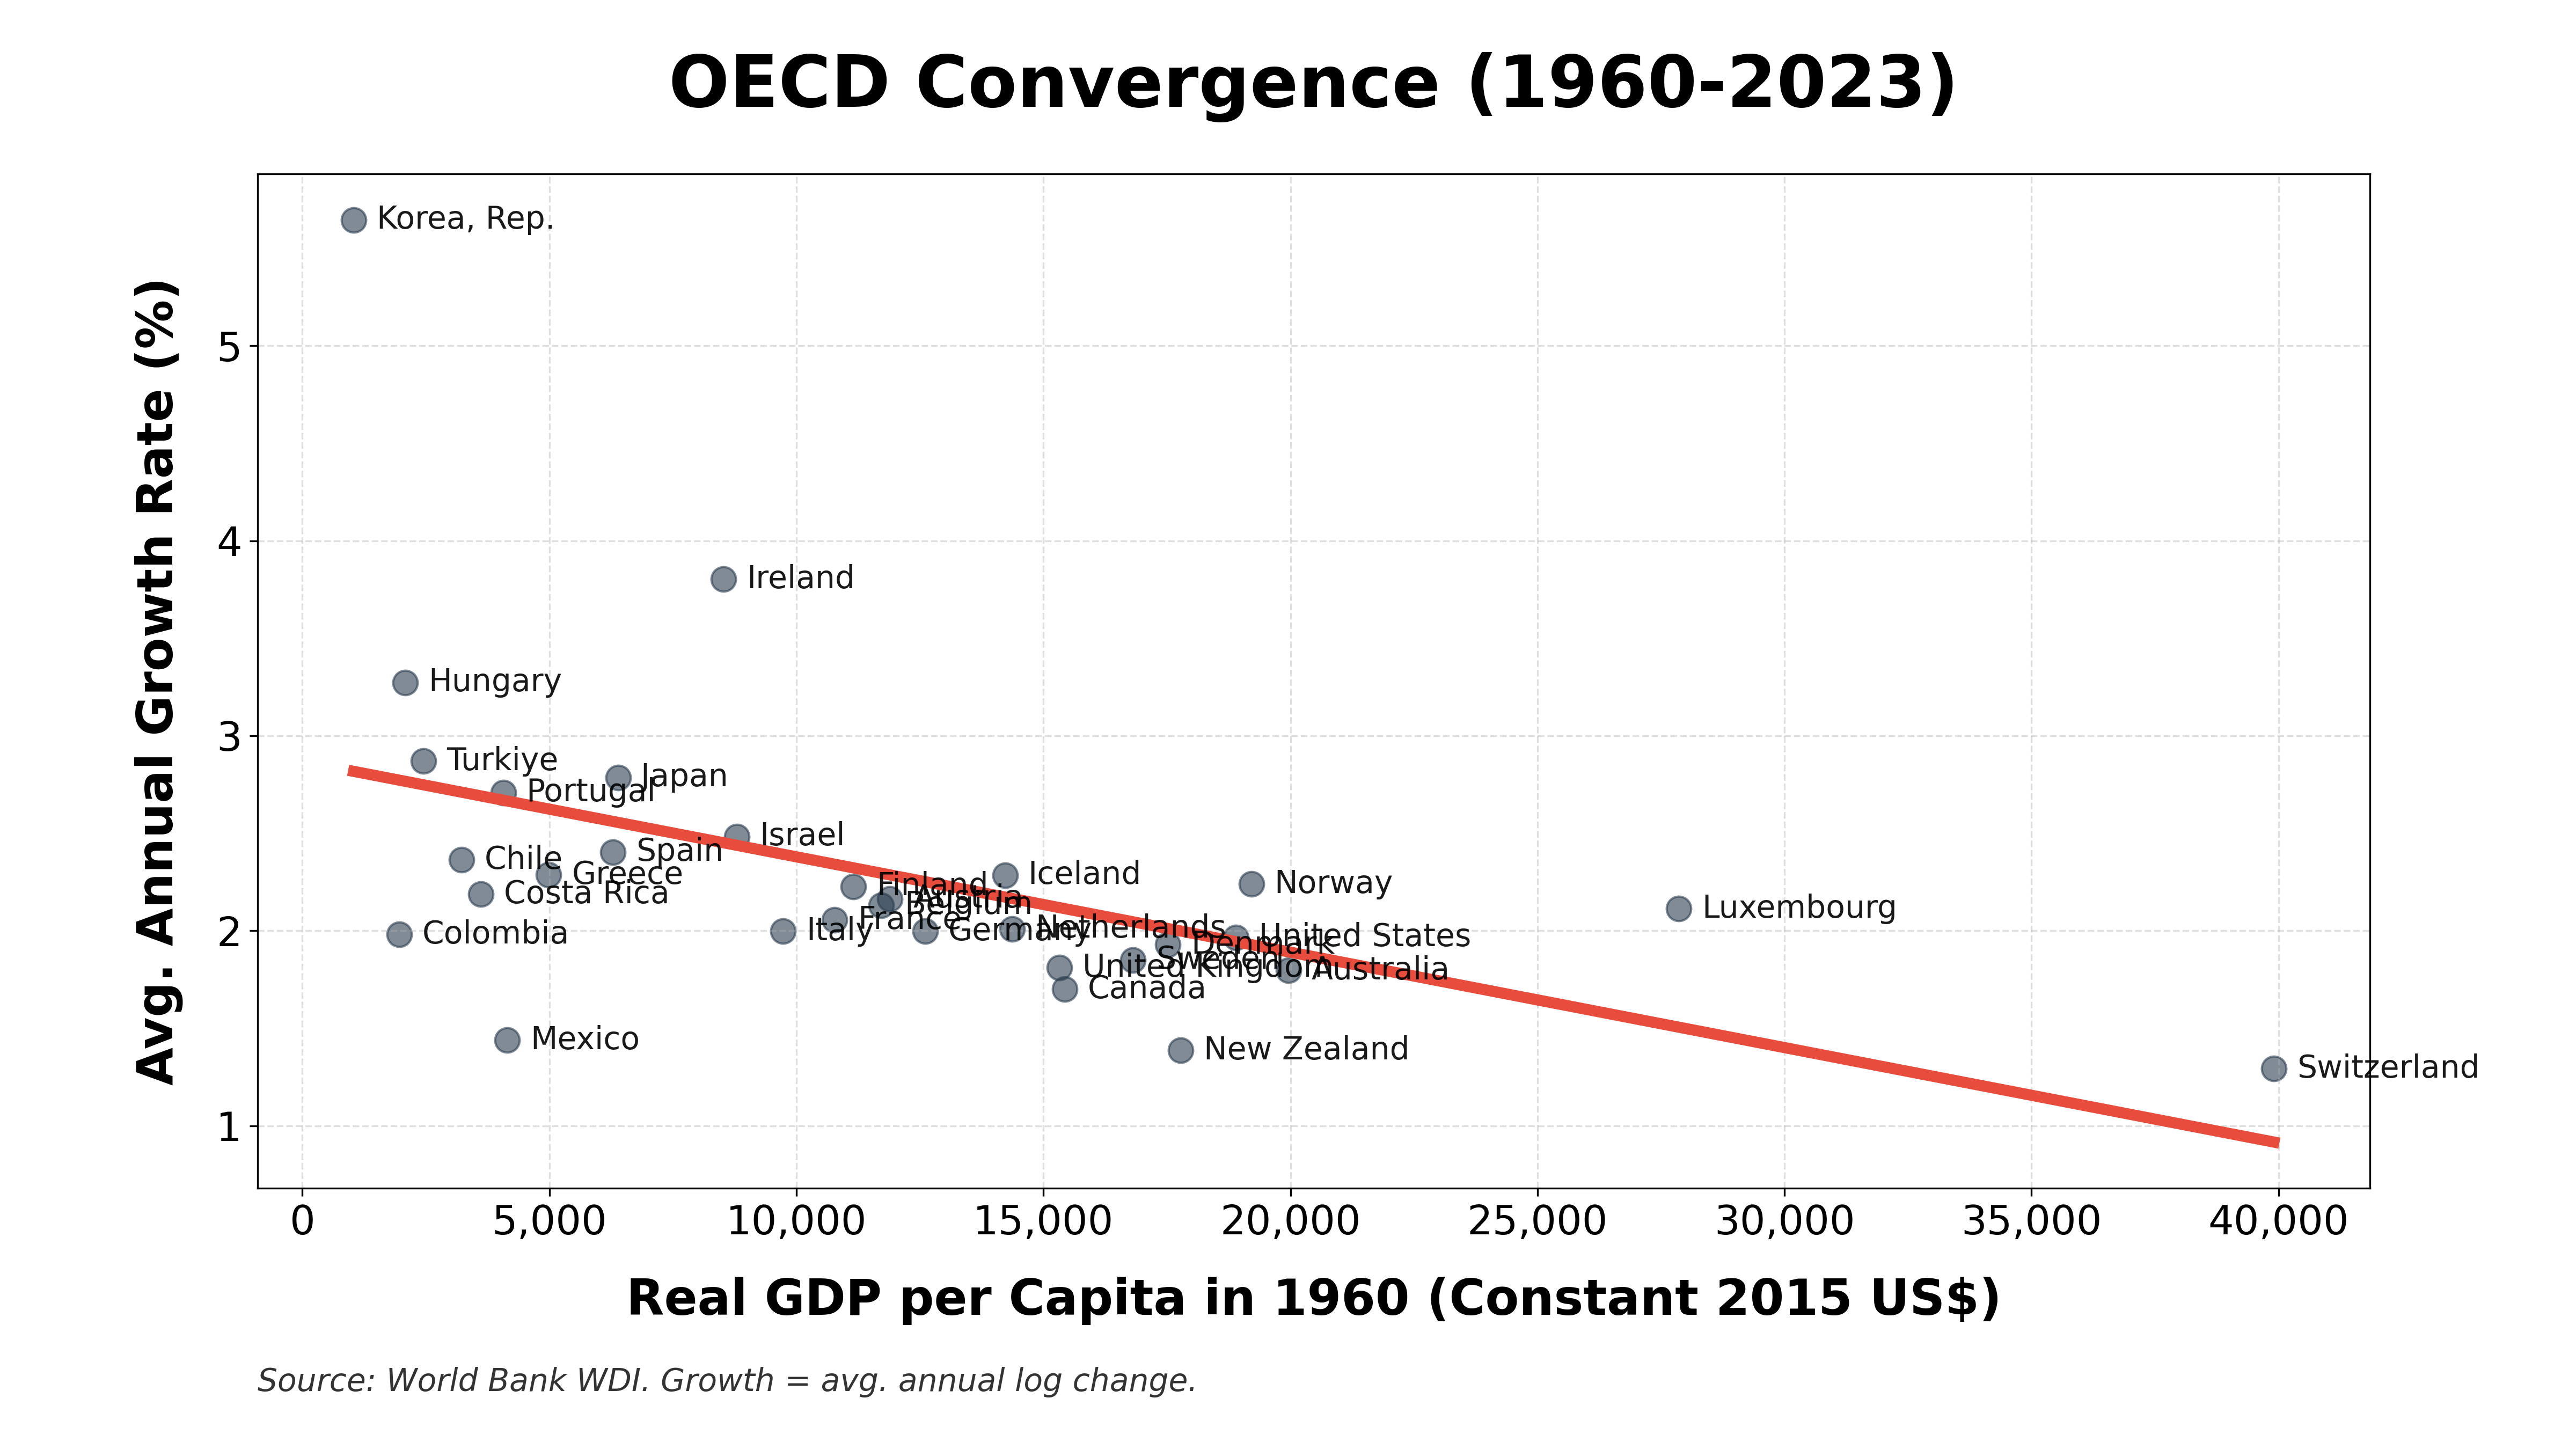
\includegraphics[scale=0.3]{figures/convergence_oecd.png}
\end{frame}

\begin{frame}{Theory vs Data}
\centering
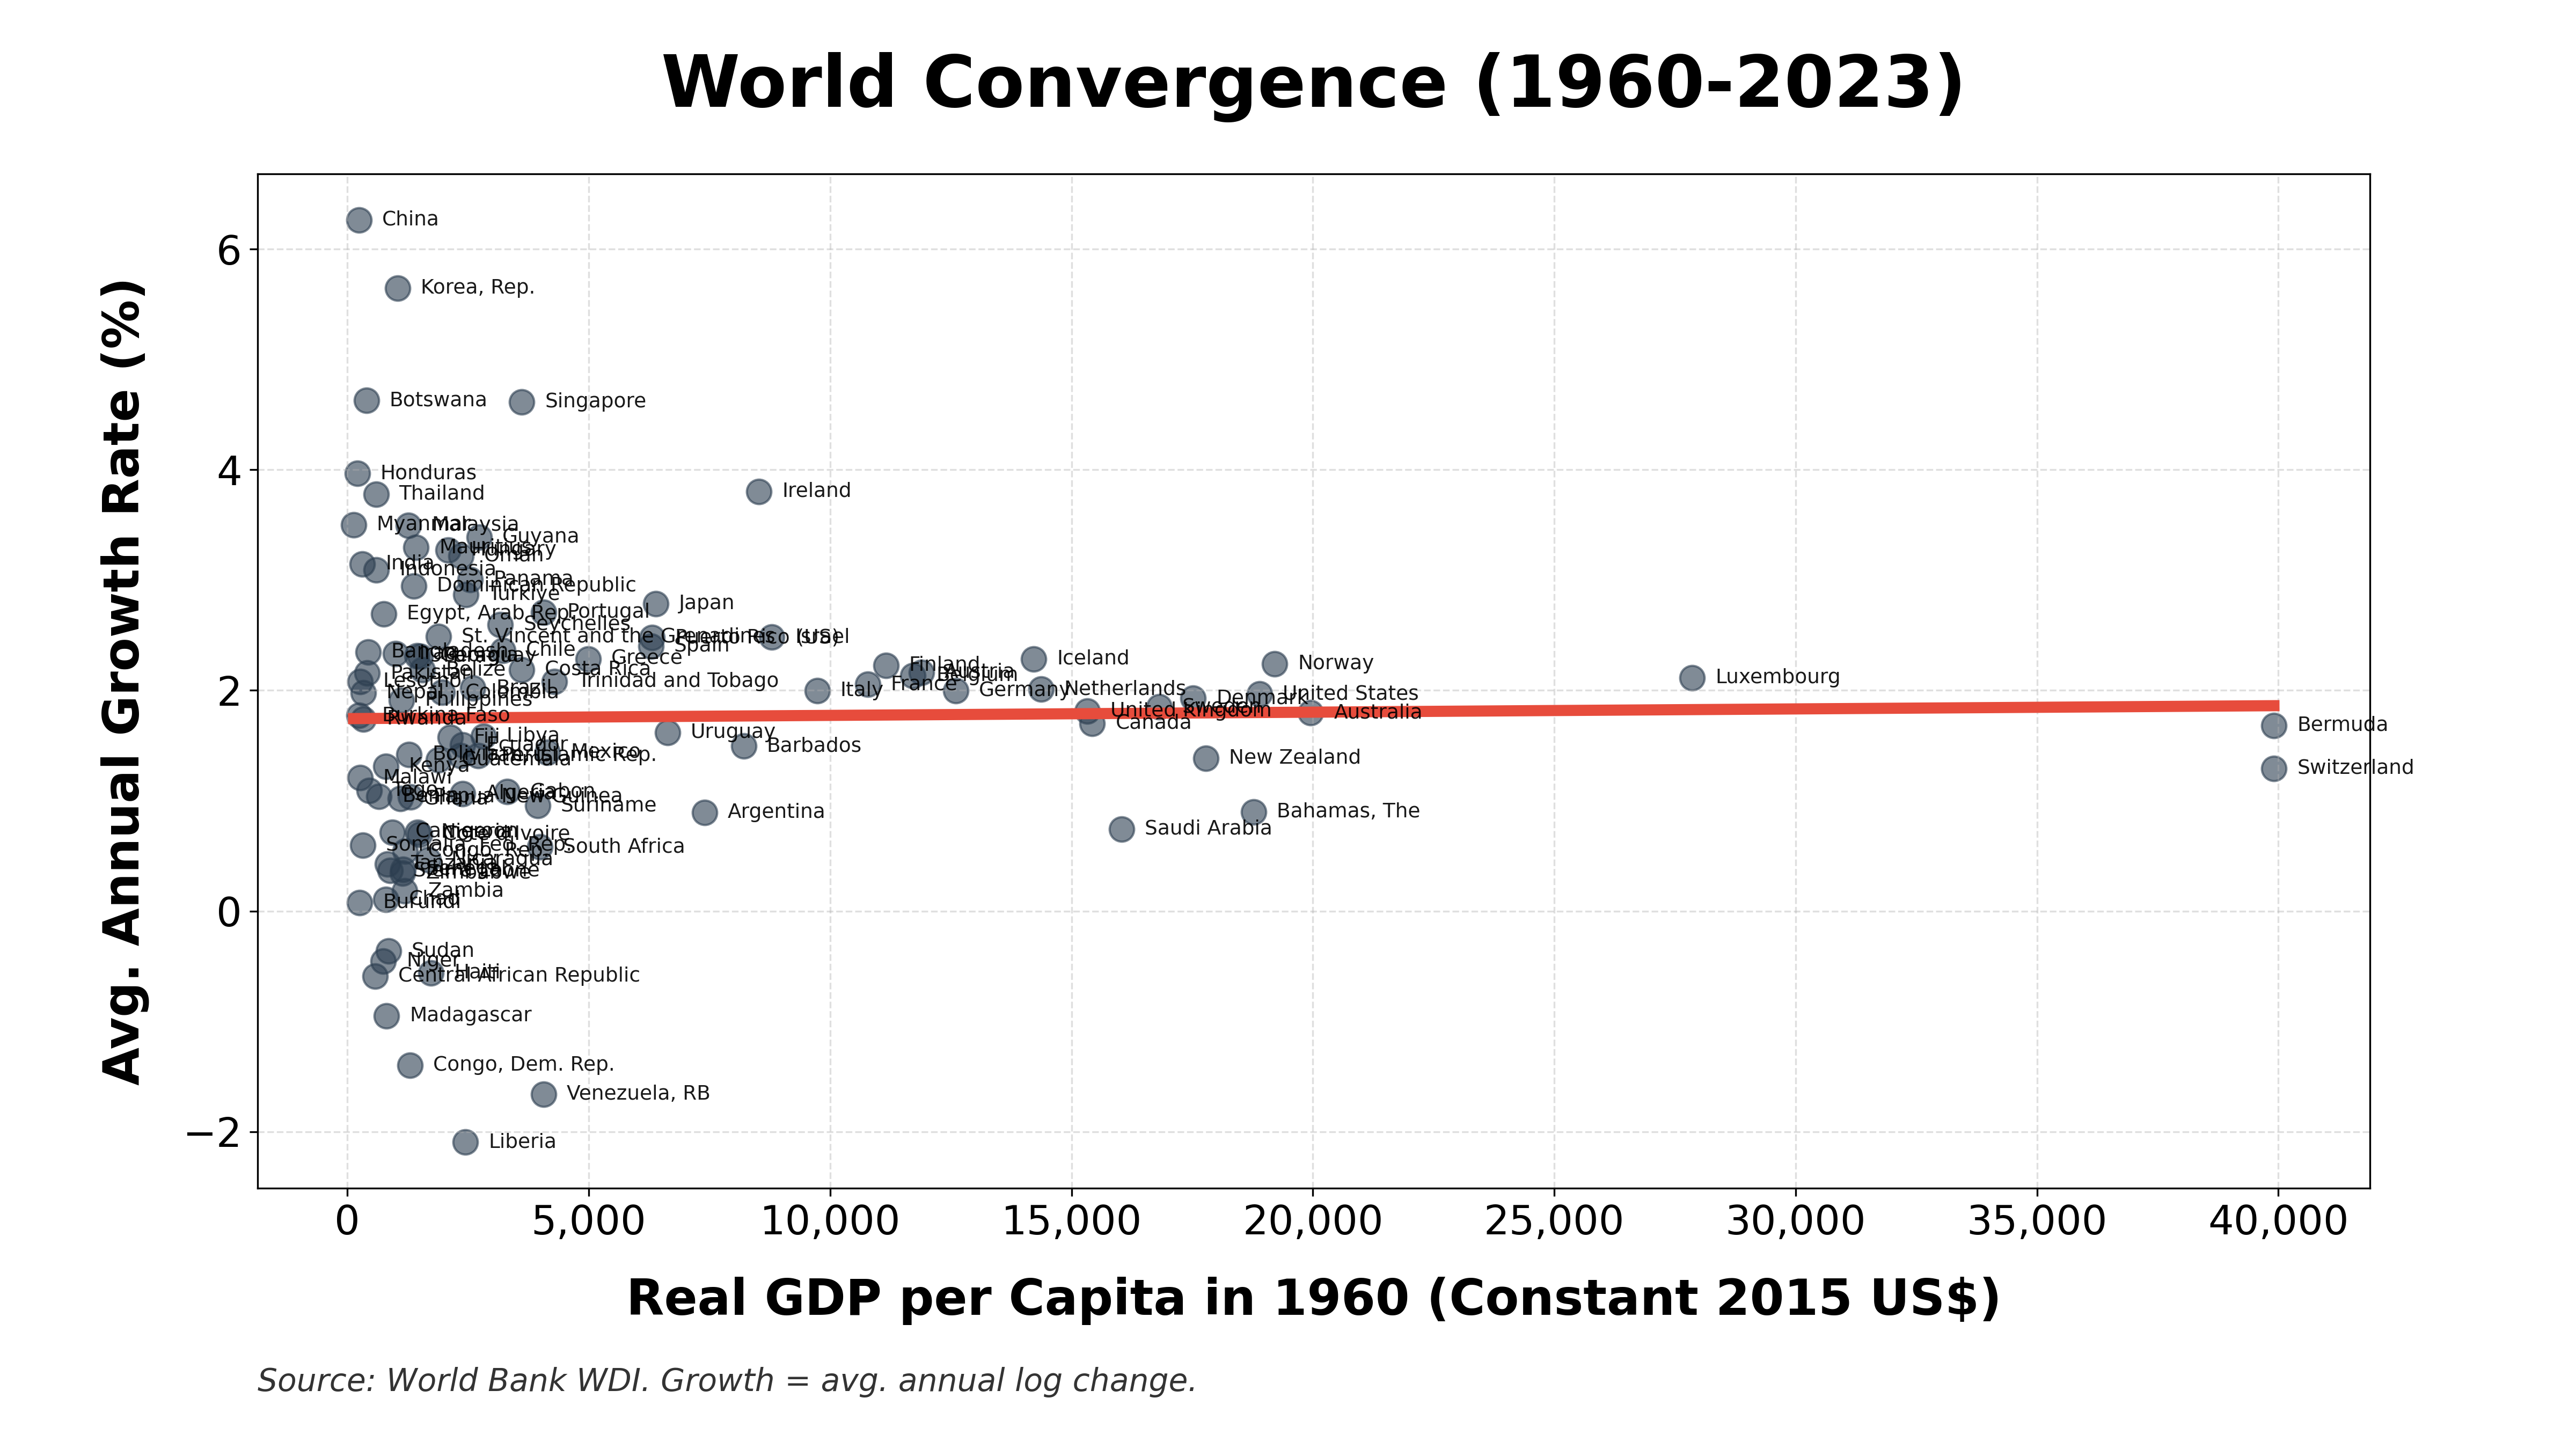
\includegraphics[scale=0.3]{figures/convergence_world.png}
\end{frame}

\begin{frame}{Case Study: Korea vs Afghanistan}
    \begin{itemize}
        \item We started the chapter by asking: Why has South Korea grown so much faster than Afghanistan in the past half century? 
        \itemvso We can apply what we have learned on transitional dynamics to try to rationalize this difference in growth performance.
        \itemvso We can think that changes in investment  and productivity have pushed South Korea to a much higher steady state than Afghanistan.
        \begin{itemize}
            \itemvso Starting from around 10 percent of U.S. income in 1960, maybe
Korea’s steady-state level moved up to 50 or 75 percent while the Afghanistan's level
remained at 10 percent.
        \end{itemize}
        \itemvso This would entail that in 1960, Korea was far below its steady state and thus had a lot of room to grow
        \itemvso Afghanistan was already close to its steady state and thus had little room to grow.
    \end{itemize}
\end{frame}

\begin{frame}{Case Study: Korea vs Afghanistan}
    \begin{itemize}
        \item What does the Solow model tell us about the determinants of the steady- state ratio
of income in South Korea to income in the United States? 
\itemvso Assuming these economies have the same rate of depreciation, the ratio of their steady- state incomes is given by:
\begin{align*}
\dfrac{y^{Korea}}{y^{US}}&=\Bigg(\dfrac{A^{Korea}}{A^{US}}\Bigg)^{3/2} \Bigg(\dfrac{s^{Korea}}{s^{US}}\Bigg)^{1/2}
\end{align*}
\end{itemize}
\end{frame}

\begin{frame}{Investment Rate: US, Korea, and Afghanistan}
\centering
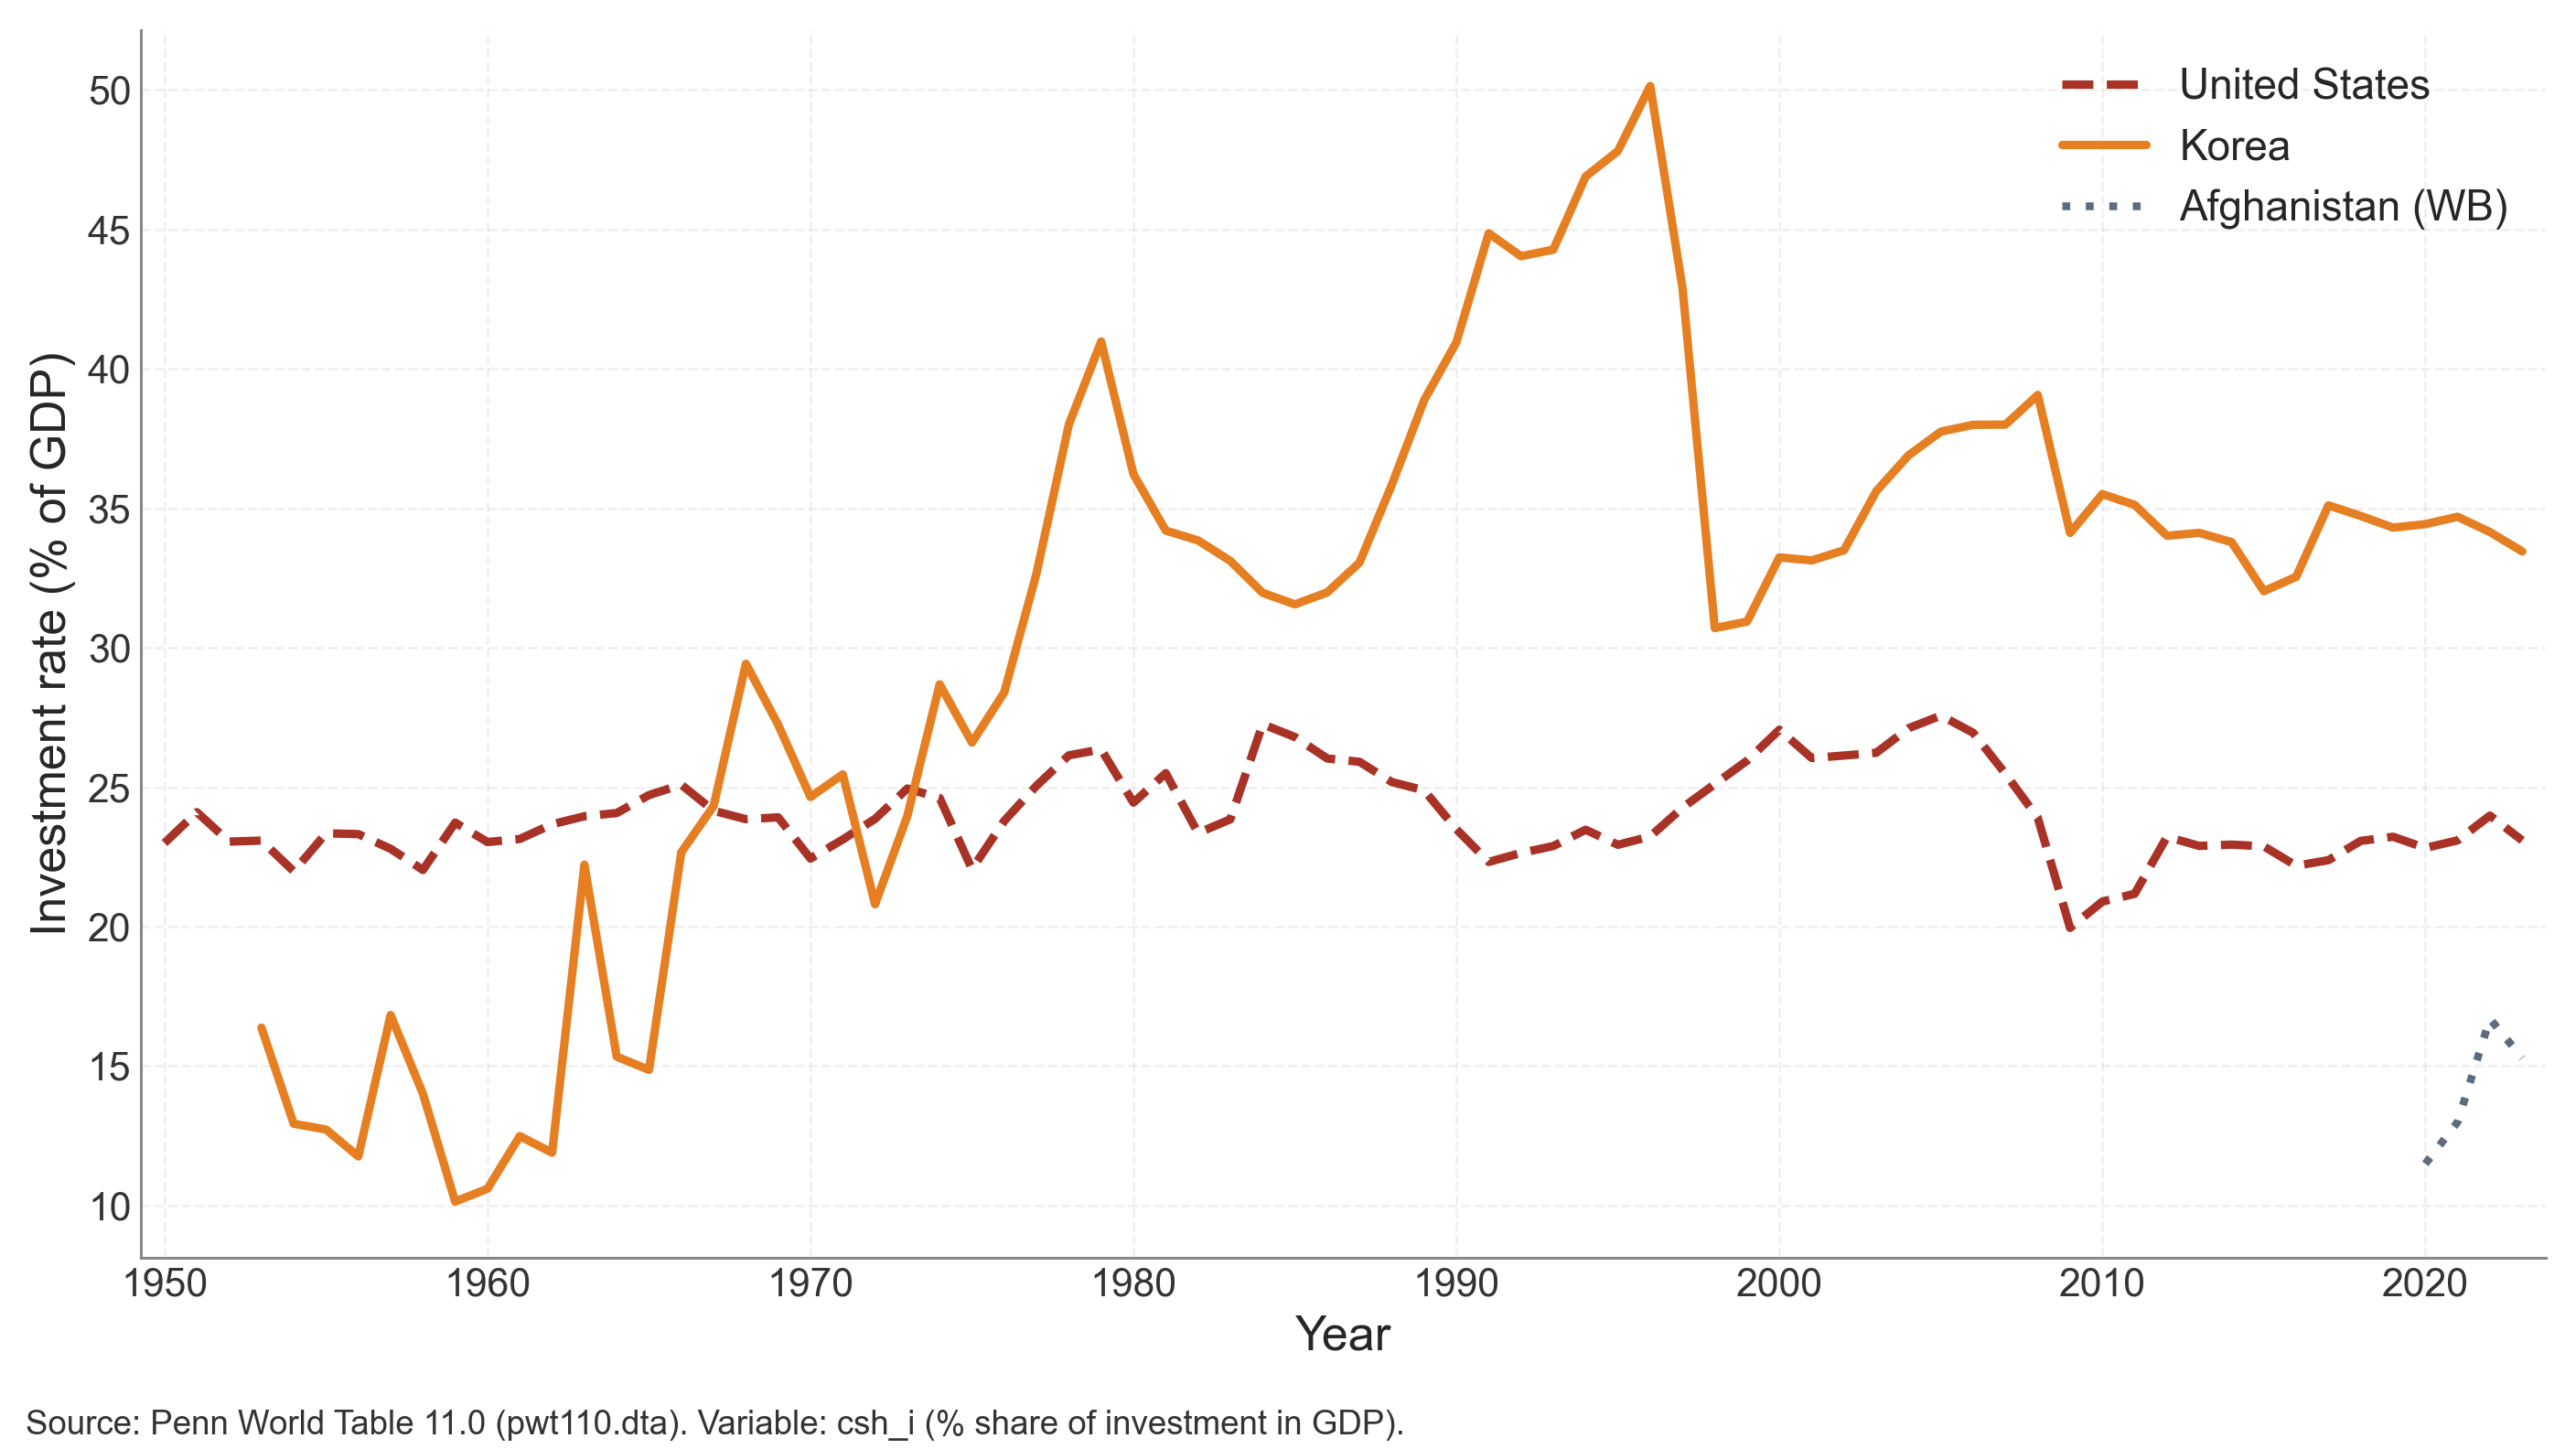
\includegraphics[width=0.98\textwidth,height=0.9\textheight,keepaspectratio]{figures/investment_rate_us_korea_pwt110.png}
\end{frame}

\begin{frame}{Case Study: Korea vs Afghanistan}
\begin{itemize}
\item  The U.S. investment rate is relatively stable
\itemvso The investment rate in Korea rises dramatically, from about 15 percent in the 1950s to around 40 percent in
the early 1990s.
\itemvso According to the Solow model, this rise should significantly increase
Korea’s steady- state income
\itemvso Transitional dynamics tells us that
the Korean economy will grow rapidly as it makes the transition to its new, higher
level.
\itemvso On the other hand, the investment rate in Afghanistan remains at much lower levels for the data that I could find.
\itemvso We could think that the steady is trapped at a low level and thus the economy has little room to grow but hopefully the recent increases in investment rate will help the country to grow faster in the future.
\end{itemize}
\end{frame}
\begin{frame}{What Does the Solow Model Teach Us?}
\begin{itemize}
\item The Solow framework is a key building block of macroeconomics of growth:
\begin{itemize}
    \item A production function with capital and labor.
    \item An accumulation equation linking saving today to capital tomorrow.
\end{itemize}
\itemvso \textbf{Strengths}:
\begin{itemize}
    \item Explains income levels in the long run (investment, TFP, depreciation).
    \item Explains growth differences through transition dynamics.
\end{itemize}
\itemvso \textbf{Limitations}:
\begin{itemize}
    \item Investment differences explain only a small part of income gaps.
    \item TFP differences remain largely unexplained.
    \item No theory of sustained long-run growth.
\end{itemize}
\itemvso Capital accumulation drives medium-run growth, but long-run growth must come from elsewhere.
\end{itemize}
\end{frame}



\begin{frame}{Beyond the Solow Model}
\begin{itemize}
    \item The Solow model does not provide a theory of long-run growth.
    \itemvso Once the economy reaches its steady state, growth stops because of decreasing returns to capital.
    \itemvso Paul Romer (1990) argued that \emph{ideas} are fundamentally different from capital and can generate non-decreasing returns.
    \itemvso Understanding this difference between ideas and capital/labor lets us build a model with long-run growth.
\end{itemize}
\end{frame}

%============================================================
\section{Increasing Returns}
%============================================================

\begin{frame}{Rival vs.\ Non-Rival Goods}
\begin{itemize}
    \item \textbf{Rival goods}: use by one agent \emph{excludes} use by another.
    \begin{itemize}
        \itemvso Examples: machines, workers, raw materials.
        \itemvso If a firm uses a machine, no other firm can use the same machine simultaneously.
    \end{itemize}
    \itemvso \textbf{Non-rival goods}: use by one agent does \emph{not} prevent use by another.
    \begin{itemize}
        \itemvso Examples: the recipe for Bolo de Bolacha from your grandmother, blueprints, software, scientific formulas.
        \itemvso Newton's laws can be applied by every scientist simultaneously.
    \end{itemize}
    \itemvso \textbf{Ideas are non-rival}: once discovered, they can be used by everyone.
\end{itemize}
\end{frame}

\section{The Romer Model}

\begin{frame}{The Romer Model: Setup}
\begin{itemize}
    \item Paul Romer (1990) developed a model of long-run growth based on the idea that ideas are non-rival goods.
    \itemvso In this model $A_t$ is going to represent the stock of ideas at time $t$.
    \itemvso In contrast to the Solow model, $A_t$ is not exogenously given and fixed, but rather it is endogenously determined by the economy and grows over time.
    \itemvso The Romer model has two sectors: a final goods sector and a research and development (R\&D) sector.
    \itemvso The final goods sector produces output using labor and ideas.
\end{itemize}
\end{frame}

\begin{frame}{The Romer Model: Setup}
\begin{itemize}
    \itemvso Final goods sector:
     \[
        Y_t = A_t\,L_Y
    \]
    Output depends on the stock of ideas $A_t$ and labor allocated to production $L_Y$.
    \itemvso R\&D sector: 
    \[
        A_{t+1}-A_t = \delta_A\,A_t\,L_A
    \]
    The production of new ideas depends on the existing stock of ideas $A_t$ and labor allocated to research $L_A$, where $\delta_A$ is a productivity parameter.

    \itemvso We assume that a constant fraction $\ell$ of the labor force ($\bar{L}$) is allocated to R\&D:
    \begin{itemize}
        \itemvso $L_Y = (1-\ell)\bar{L}$
        \itemvso $L_A = \ell \bar{L}$
        \itemvso Total labor constraint: $L_Y + L_A = \bar{L}$
    \end{itemize}
\end{itemize}
\end{frame}


\begin{frame}{Solution of the Romer Model}
    \begin{itemize}
        \item Output per person:
        \[
        y_t = \frac{Y_t}{\bar{L}} = A_t (1-\ell)
        \]
        \item Growth rate of ideas:
        \[
        g_A = \frac{A_{t+1}-A_t}{A_t} = \delta_A L_A = \delta_A \ell \bar{L}
        \]
        The growth rate of ideas is going to depend on
            \begin{itemize}
                \itemvso the number of researchers: $L_A = \ell \bar{L}$
                \itemvso the productivity of research: $\delta_A$
            \end{itemize} 
        \itemvso Ouput per person also grows that the same constant rate.\\
        \vspace{0.5cm}
        $\Rightarrow$ \textbf{A Theory of Sustained Growth}
    \end{itemize}
    
\end{frame}

\begin{frame}{Why there is sustained growth in the Romer model?}
    \begin{itemize}
        \item In Solow, the accumulation of capital runs into diminishing returns: each additional unit of capital adds less and less to output.
        \itemvso Eventually, investment only offsets depreciation and growth stops.
        \itemvso In Romer, the accumulation of ideas does not run into diminishing returns:
        \begin{align*}
        A_{t+1}-A_t &= \delta_A A_t L_A
        \end{align*}
        \vspace{-0.6cm}
        \item As we accumulate more knowledge, the return to knowledge does not fall.
        \itemvso Old ideas continue to help us produce new ideas in a virtuous circle that sustains economic growth.
    \end{itemize}
\end{frame}

\subsection{Experiments in the Romer Model}
\begin{frame}{Lower Population}
\begin{itemize}
    \item A decrease in population $\bar{L} \rightarrow \tilde{L}$ decreases the number of researchers $L_A = \ell \bar{L}$, which slows down the growth rate of ideas $\tilde{g}_A = \delta_A \ell \tilde{L}$.
    \itemvso This is the \textbf{scale effect}: larger economies grow faster because they have more researchers.
\end{itemize}

\begin{center}

\begin{tikzpicture}
    \begin{axis}[
        width=6.5cm, height=4cm,
        xmin=0, xmax=10,
        ymin=0, ymax=12,
        xtick={0,3.3,10},
        xticklabels={$t_0$,$t^*$,$t$},
        ytick=\empty,
        ylabel={},
        xlabel={Time},
        axis lines=left,
        title={\textbf{Population}},
        domain=0:10,
        samples=2,
        thick,
    ]
    % Actual population with shock
    \addplot[blue, thick] coordinates {(0,10) (3.3,10)};
    \addplot[blue, thick] coordinates {(3.3,10) (3.3,5)};
    \addplot[blue, thick] coordinates {(3.3,5) (10,5)};
    \addplot[only marks, mark=*, blue] coordinates {(3.3,10) (3.3,5)};
    % Counterfactual: population stays high (dashed)
    \addplot[blue, dashed, thick] coordinates {(0,10) (10,10)};
    \end{axis}
\end{tikzpicture}
\qquad
\begin{tikzpicture}
    \begin{axis}[
        width=6.5cm, height=4cm,
        xmin=0, xmax=10,
        ymin=2, ymax=3.2,
        xtick={0,3.3,10},
        xticklabels={$t_0$,$t^*$,$t$},
        ytick=\empty,
        ylabel={},
        xlabel={Time},
        axis lines=left,
        title={\textbf{Log Output per Person}},
        domain=0:10,
        samples=100,
        thick,
    ]
    % Actual: fast initial growth, then slower after shock (lower trend)
    % Before shock: log(y) = 2.2 + 0.08*x
    \addplot[red, thick, domain=0:3.3] {2.2 + 0.08*x};
    % After shock: log(y) = value at shock + 0.03*(x-3.3)
    \addplot[red, thick, domain=3.3:10] {2.2 + 0.08*3.3 + 0.03*(x-3.3)};
    \addplot[only marks, mark=*, red] coordinates {(3.3,{2.2 + 0.08*3.3})};
    % Counterfactual: always fast growth (dashed)
    \addplot[red, dashed, thick, domain=0:10] {2.2 + 0.08*x};
    \end{axis}
\end{tikzpicture}

\end{center}
\end{frame}


\begin{frame}{Higher Fraction of Researchers}
\begin{itemize}
    \item An increase in the fraction of researchers $\ell \rightarrow \tilde{\ell}$ increases the growth rate of ideas $\tilde{g}_A = \delta_A \tilde{\ell} \bar{L}$ and output.
    \itemvso But as people are allocated to research, less people are allocated to production, so the level of output per person falls.
    \itemvso Increasing the research share involves a trade-off.
\end{itemize}
\begin{center}
    \begin{tikzpicture}
        \begin{axis}[
            width=6.5cm, height=4cm,
            xmin=0, xmax=10,
            ymin=0, ymax=1,
            xtick={0,3.3,10},
            xticklabels={$t_0$,$t^*$,$t$},
            ytick=\empty,
            ylabel={},
            xlabel={Time},
            axis lines=left,
            title={\textbf{Fraction of Researchers}},
            domain=0:10,
            samples=2,
            thick,
        ]
        % Actual: increase in fraction of researchers
        \addplot[blue, thick] coordinates {(0,0.2) (3.3,0.2)};
        \addplot[blue, thick] coordinates {(3.3,0.2) (3.3,0.4)};
        \addplot[blue, thick] coordinates {(3.3,0.4) (10,0.4)};
        \addplot[only marks, mark=*, blue] coordinates {(3.3,0.2) (3.3,0.4)};
        % Counterfactual: fraction stays low (dashed)
        \addplot[blue, dashed, thick] coordinates {(0,0.2) (10,0.2)};
        \end{axis}
    \end{tikzpicture}
        \qquad
    \begin{tikzpicture}
        \begin{axis}[
            width=6.5cm, height=4cm,
            xmin=0, xmax=10,
            ymin=2, ymax=3.2,
            xtick={0,3.3,10},
            xticklabels={$t_0$,$t^*$,$t$},
            ytick=\empty,
            ylabel={},
            xlabel={Time},
            axis lines=left,
            title={\textbf{Log Output per Person}},
            domain=0:10,
            samples=100,
            thick,
        ]
        % Before increase: log(y) = 2.2 + 0.05*x
        \addplot[red, thick, domain=0:3.3] {2.2 + 0.05*x};
        % Drop at t^*: subtract 0.2 from the level
        \addplot[red, thick, domain=3.3:10] {2.2 + 0.05*3.3 - 0.2 + 0.1*(x-3.3)};
        % Mark the drop
        \addplot[only marks, mark=*, red] coordinates {(3.3,{2.2 + 0.05*3.3})};
        \addplot[only marks, mark=*, red] coordinates {(3.3,{2.2 + 0.05*3.3 - 0.2})};
        % Counterfactual: always low growth (dashed)
        \addplot[red, dashed, thick, domain=0:10] {2.2 + 0.05*x};
        % Vertical dashed line to show the drop
        \addplot[red, dashed] coordinates {(3.3,{2.2 + 0.05*3.3}) (3.3,{2.2 + 0.05*3.3 - 0.2})};
        \end{axis}
    \end{tikzpicture}
\end{center}
\end{frame}

\section{Conclusion}
\begin{frame}{Conclusion}
    \begin{itemize}
        \item The Solow model explains medium-run growth through capital accumulation, but long-run growth must come from elsewhere.
        \itemvso The Romer model provides a theory of sustained long-run growth.
        \itemvso Because ideas are nonrivalrous, it is not ideas per person that matter, but rather this total stock of ideas.
        \itemvso Increases in the stock of knowledge lead to sustained economic growth for countries that have access to that knowledge.
    \end{itemize}
    
\end{frame}


\end{document}
